\documentclass[a4paper,12pt]{article}
\usepackage{fullpage}
\usepackage{amsmath,amsthm,amsfonts,amssymb,amscd}
\usepackage{xcolor}
\usepackage{graphicx}
\usepackage{xepersian}
\usepackage{placeins}


\newcommand{\StudentOne}{4011262134}
\newcommand{\StudentTwo}{4011262098}
\newcommand{\NameOne}{مینا جمشیدی}
\newcommand{\NameTwo}{مبینا محمدی}
\newcommand{\ProjectName}{مستندات پروژه NLP}


\definecolor{CustomBackground}{HTML}{1C1C1C}
\pagecolor{CustomBackground}
\color{white}


\settextfont{Vazir.ttf}[
BoldFont = Vazir-Bold.ttf, 
Path = fonts/]
\setlatintextfont{Vazir.ttf}[
BoldFont = Vazir-Bold.ttf, 
Path = fonts/]


\renewcommand{\baselinestretch}{1.2}
\let\nobreaksection\section
\renewcommand{\section}{\nobreaksection} 

\begin{document}
	

	\hrule \medskip
	\begin{minipage}{0.3\textwidth}
		\raggedright
		\small
		\NameOne \\
		\StudentOne \\
		\NameTwo \\
		\StudentTwo
	\end{minipage}
	\begin{minipage}{0.4\textwidth} 
		\centering 
		\large\bfseries
		\ProjectName \\
	\end{minipage}
	\begin{minipage}{0.3\textwidth}
		\raggedleft
		\small
	\end{minipage}
	\medskip\hrule 
	\vspace*{1.5cm}  
	

\section{فاز اول: استخراج ویژگی‌ها}

	
	\subsection{چالش‌های داده‌های خام}
	\begin{itemize}
		\item وجود نویزهایی مانند نشانی‌های وب، ایمیل، علائم نگارشی و تکرار حروف
		\item شامل بودن کلمات پرتکرار (stopwords) که اطلاعات مفیدی منتقل نمی‌کنند
		\item وجود کلمات با فرمت‌های گرامری متفاوت (مانند run، running، ran) که باید به یک ریشه نگاشته شوند
		\item وجود حروف بزرگ/کوچک که می‌توانند مدل را دچار سردرگمی کنند (مثلاً \texttt{Apple} با \texttt{apple} متفاوت تفسیر شود)
	\end{itemize}
	
	\subsection{راهکارها و منطق انتخاب‌شده}
دلایل هر تکنیک استفاده شده:
	
	\begin{itemize}
		\item \textbf{تبدیل به حروف کوچک (lowercase):} برای یکسان‌سازی نوشتار کلمات و جلوگیری از تکرار غیر ضروری ویژگی‌ها.
		
		\item \textbf{حذف لینک‌ها و ایمیل‌ها:} این اطلاعات معمولاً حاوی معنای خاصی برای دسته‌بندی محصول نیستند و حذف آن‌ها به ساده‌سازی متن کمک می‌کند.
		
		\item \textbf{حذف اعداد:} اعداد در این نوع مسئله‌ها معمولاً کاربرد خاصی ندارند (مثلاً شماره مدل یا سایز)، بنابراین حذف شدند مگر اینکه در تحلیل آینده به صورت جدا استفاده شوند.
		
		\item \textbf{حذف علائم نگارشی و HTML:} این کار برای کاهش نویز و تمرکز بر محتوای متنی اصلی انجام شد.
		
		\item \textbf{کاهش کشیدگی کلمات:} کلماتی مثل \texttt{soooo} به \texttt{soo} تبدیل شدند تا مدل دچار تکرار بی‌مورد نشود.
		
		\item \textbf{حذف کلمات توقف (Stopwords):} کلماتی مثل \texttt{the, is, in} اطلاعات خاصی منتقل نمی‌کنند و حضور آن‌ها باعث می‌شود مدل یادگیری سخت‌تری داشته باشد.
		
		\item \textbf{Lemmatization:} برای تبدیل کلمات به شکل پایه‌شان (مثل \texttt{running} به \texttt{run}) از Lemmatizer استفاده شد. این کار به مدل کمک می‌کند مفهوم اصلی کلمه را فارغ از فرم گرامری‌اش یاد بگیرد.
		
		\item \textbf{توکن‌سازی:} برای پردازش بهتر، متن به کلمات جداگانه شکسته شد تا بتوان روی هر کلمه عملیات انجام داد.
	\end{itemize}
	

	در پایان هر نمونه متنی به یک نسخه تمیز، یکنواخت و کاهش‌یافته از نظر اطلاعات زائد تبدیل شد. این داده‌ها اکنون آماده‌اند تا در مراحل بعدی برای برداری‌سازی (با TF-IDF و Word2Vec) استفاده قرار گیرند.
	\begin{figure}[h]
		\centering
		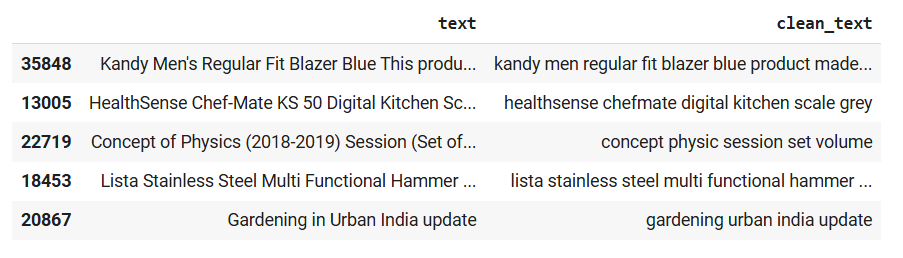
\includegraphics[width=1\textwidth]{1.png}
	\end{figure}
	\FloatBarrier
	
	\section{فاز دوم: بردارسازی متون با استفاده از TF-IDF }
	

	در این بخش، الگوریتم TF-IDF بدون استفاده از هیچ کتابخانه‌ای پیاده‌سازی شد. 
	
	\subsection{چالش‌ها و راهکارها}
	\begin{itemize}
		\item \textbf{محاسبه DF:} یکی از چالش‌ها، محاسبه دقیق Document Frequency برای هر واژه بود، به طوری که شمارش تکرار یک واژه فقط یک‌بار در هر سند لحاظ شود. برای حل این مسئله، از \lr{set} استفاده شد تا کلمات تکراری در هر سند فقط یک‌بار شمرده شوند.
		
		\item \textbf{جلوگیری از تقسیم بر صفر:} در محاسبه IDF، برای جلوگیری از تقسیم بر صفر در فرمول \lr{$\log(N / df)$}، یک واحد به \lr{df} اضافه شد، یعنی از \lr{$\log(N / (1 + df))$} استفاده شد.
		
		\item \textbf{ابعاد ماتریس:} با توجه به تعداد واژگان یکتا (واژگان نهایی)، لازم بود که ابتدا دیکشنری \lr{word2idx} تعریف شود تا اندیس هر واژه در ماتریس TF-IDF مشخص شود. سپس یک ماتریس $N \times V$ (تعداد اسناد $\times$ تعداد واژگان) ساخته شد.
		
	\end{itemize}
	
	\subsection{نتایج}
	نتیجه داکیومنت اول نشان داد که واژگانی مانند \lr{kandy}، \lr{velvet} و \lr{buttoned} دارای مقادیر TF-IDF بالاتری نسبت به کلمات عمومی‌تر مانند \lr{product} یا \lr{made} هستند. این نشان می‌دهد که TF-IDF به درستی کلمات متمایزکننده را نسبت به کلمات پرتکرار تشخیص داده است.
		\begin{figure}[h]
		\centering
		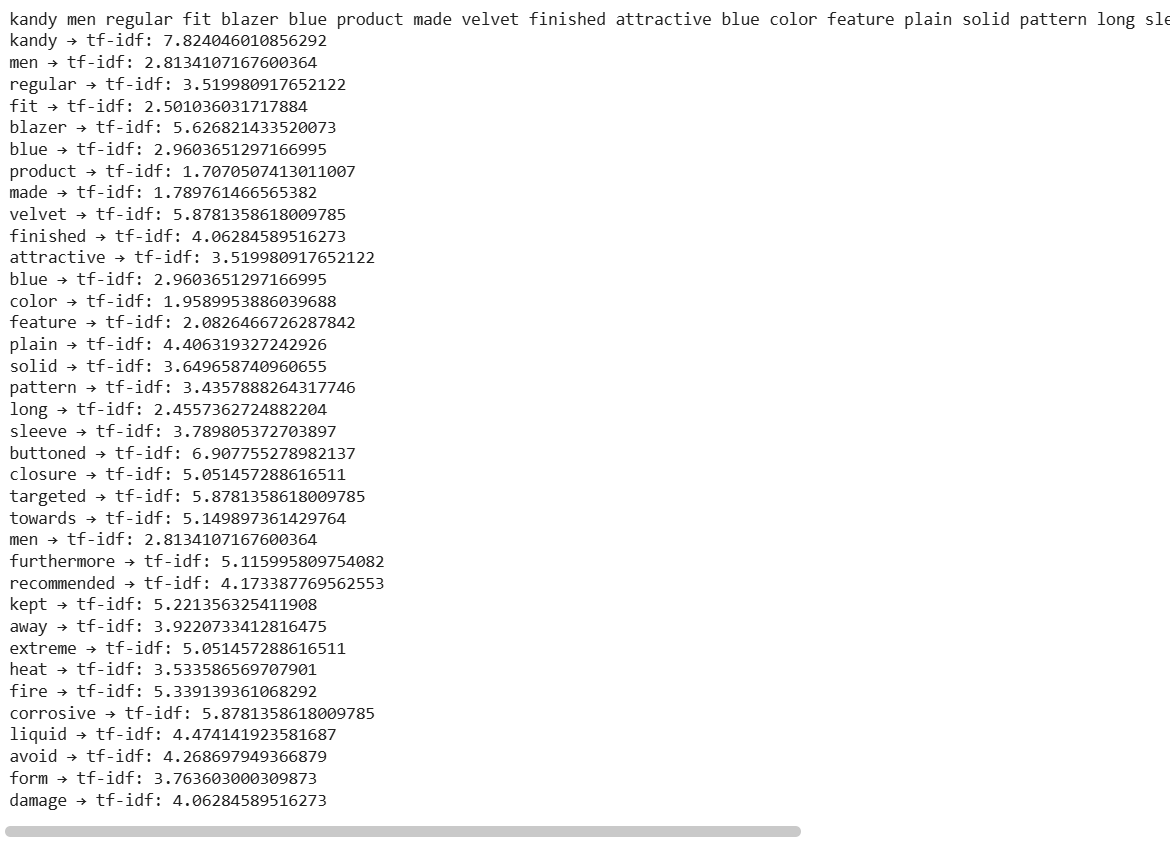
\includegraphics[width=1\textwidth]{2-1.png}
	\end{figure}
	\FloatBarrier
	
	\section{فاز دوم: بردارسازی متون با استفاده از Word2Vec}
	 از مدل \lr{Word2Vec} کتابخانه \lr{gensim} استفاده شد.
	
	\subsection{چالش‌ها و تصمیمات}
	\begin{itemize}
		\item \textbf{توکن‌سازی دقیق:} برای آموزش Word2Vec نیاز به توکن‌سازی دقیق داشتیم. در ابتدا از \lr{split()} استفاده شد، اما برای نتایج بهتر از \lr{word\_tokenize} از کتابخانه \lr{nltk} استفاده شد.
		
		\item \textbf{تنظیمات مدل:} برای آموزش مدل، پارامترهایی مانند \lr{vector\_size=100}، \lr{window=5} و \lr{min\_count=2} انتخاب شد. این تنظیمات با توجه به اندازه داده‌ها و برای جلوگیری از نویز ناشی از کلمات بسیار کم‌تکرار انجام شد.
		
		\item \textbf{کلمات نادیده گرفته‌شده:} برخی کلمات به دلیل \lr{min\_count} وارد مدل نمی‌شوند، بنابراین در تحلیل نهایی ممکن است برخی واژه‌ها بردار نداشته باشند.
	\end{itemize}
	
	\subsection{نتایج}
	با بررسی بردار کلمه \lr{painting} مشاهده شد که شباهت زیادی با واژگان مفهومی مانند \lr{art}، \lr{drawing}، و \lr{craft} دارد. این نشان می‌دهد که مدل Word2Vec توانسته ارتباط معنایی بین کلمات را تا حد مناسبی بیاموزد. همچنین خروجی بردار عددی کلمه \lr{painting} به‌خوبی ساختار توزیعی مدل را نشان می‌دهد.
		\begin{figure}[h]
		\centering
		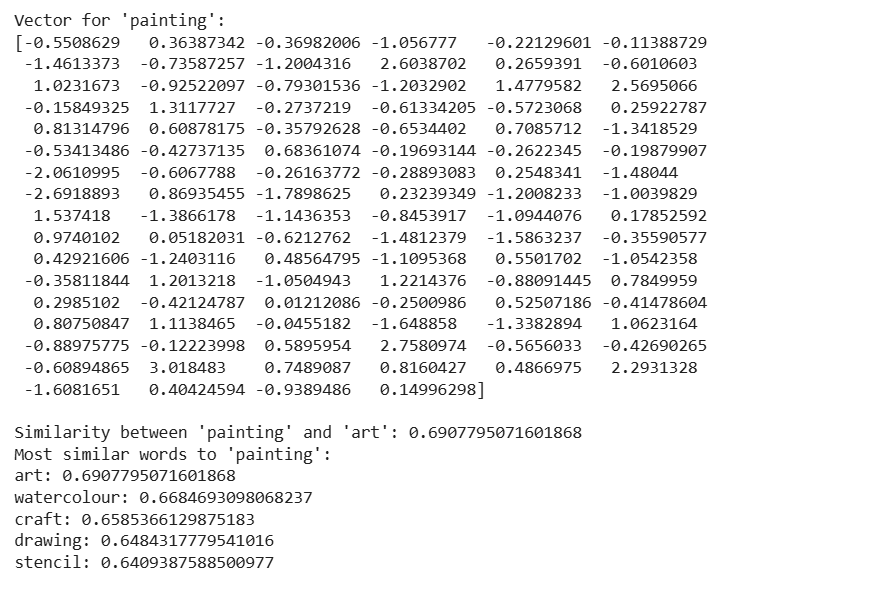
\includegraphics[width=1\textwidth]{2-2.png}
	\end{figure}
	\FloatBarrier
	
	
	

\end{document}